% One-page research summary for outreach.  Build:  cd paper/summary && tectonic one_page.tex
\documentclass[10pt]{article}
\usepackage[a4paper,margin=0.7in,top=0.55in,bottom=0.55in]{geometry}
\usepackage[T1]{fontenc}
\usepackage{lmodern}
\usepackage{microtype}
\usepackage{amsmath}
\usepackage{graphicx}
\usepackage{xcolor}
\usepackage[hidelinks]{hyperref}
\usepackage{enumitem}
\setlist{nosep,leftmargin=1.1em,topsep=1pt}
\setlength{\parindent}{0pt}
\setlength{\parskip}{3pt}
\pagestyle{empty}
\newcommand{\sect}[1]{\vspace{3pt}{\large\bfseries #1}\par\vspace{1pt}}
\definecolor{reg}{HTML}{1F6F43}
\newcommand{\reg}{\textcolor{reg}{\textsc{pre-registered}}}

\begin{document}
{\LARGE\bfseries The retrain never saw the label}\\[2pt]
{\large An ill-posed reference in class-unlearning audits of conditional diffusion models}\\[3pt]
Arush Badhe \,$\cdot$\, research summary, November 2026\\ Paper, code, data and pre-registrations: \href{https://github.com/Arubad/unlearning-audit}{\texttt{github.com/Arubad/unlearning-audit}}

\sect{Problem}
Machine-unlearning methods for diffusion models are judged against an \emph{exact retrain}, a model trained from scratch without the forgotten class. This is often done by comparing the two \emph{under the forgotten label}: losses, generation rates, or FID against one retrain (e.g.\ FID$_O$, Zheng, Tai \& Yeh, CVPR 2026, which reports $0.00$ for the retrain). We asked whether that reference is well-posed.

\sect{Finding}
It is not. When the class label enters through a learned embedding, the default in DiT, ADM and EDM code, a retrain never sees the forgotten label, so that label's embedding row gets \emph{exactly zero gradient} and stays at its random initialisation. A retrain's ``behaviour on the forgotten class'' is each network's reading of an untrained, seed-specific random vector, and independent retrains disagree. Querying instead through the \emph{null} (classifier-free-guidance) label, which every model trains, gives a calibrated reference.

\sect{Evidence}
\small CIFAR-10 class-conditional DDPM (6.5M params); 3 exact retrains for each of 4 classes; five studies registered before data, with outcomes reported whether or not they held.\normalsize
\begin{itemize}
\item \textbf{Untrained row:} 12/12 retrains, row unchanged to float32 round-off ($\le3.4\cdot10^{-6}$).
\item \textbf{Removed-label reference fails:} a held-out retrain should score $1$; it scores $-2.1$ to $2.2$ or is undefined (7/12), and fails on every class. \reg{} on 2 new classes. Sharing one row across retrains does not fix it; our registered predictions for that test \emph{failed}, and we changed our explanation.
\item \textbf{Null-label reference works:} held-out retrains score $0.94$--$1.13$ (9/9 in the registered band) on the 3 classes with enough signal; retrains that removed a different class score $<0.2$. \reg{}; one registered homogeneity rule failed.
\item \textbf{The audit can be gamed in zero steps:} re-drawing only the forgotten row (no training) passes the removed-label audit on 30--60\% of draws, a rate similar to genuine retrains (3/9). Yet re-fitting that one row restores the class to ${\ge}95.5\%$ of samples, against ${\le}24.5\%$ for retrains. \reg{} (pass rates); exploratory (re-fit).
\item \textbf{The published metric inherits it:} with FID$_O$ computed as defined, two exact retrains differ by $2.1$--$4.3\times$ the sampling floor, the size of published method scores; the forgotten label inflates this $1.3$--$3.0\times$. On 2 of 3 classes the \emph{unmodified} model is no farther from some retrain than the retrains are from each other. \reg{}; our sanity rule failed on 2 classes, held on 1.
\end{itemize}

\vspace{-2pt}
\begin{center}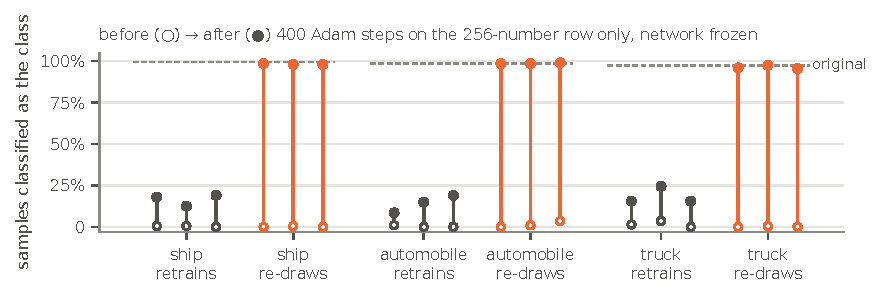
\includegraphics[width=0.86\linewidth]{../figures/fig4_row_refit.pdf}\\[-2pt]
{\footnotesize Re-fitting only the forgotten label's 256-number row (network frozen) restores the class in zero-step re-draws that \emph{passed} the audit, but not in exact retrains.}\end{center}
\vspace{-4pt}

\sect{Status and limits}
A 4-page workshop paper, code, unit-tested scoring for every registered rule, and the full run log are public. Main limits: \emph{one small architecture on CIFAR-10}, three retrains per class, and generality to DiT/ADM/EDM argued from their code, not trained.

\sect{Proposed next step, and what I am asking for}
Test the finding on a \textbf{small DiT} (plus an EDM-style label input) with 4 retrains per class, under rules registered before any data; a negative result would also be reported. The design is written and in the repository; it needs \textbf{${\approx}70$--$140$ T4 GPU-hours}, beyond my free quota. I am looking for \textbf{research guidance} to turn this into a full publication, and \textbf{help with compute} for this experiment.
\end{document}
